\documentclass[professionalfont,10pt]{beamer}
\usetheme{Pavlo}				% My custom theme

\usepackage{newtxtext} % For Times New Roman font
\usepackage[utf8]{inputenc}
\usepackage[T1]{fontenc}
%Information to be included in the title page:
\title{Introduction to Gaussian Process Regression as Ordinary Kriging}
\subtitle{A Brief Overview Presentation}
\author{Pavlo Vlastos}
%\date{August 25th, 2020}
\institute{Autonomous Systems Laboratory \\ The University of California at Santa Cruz}
\titlegraphic{
\includegraphics[width=2.5cm]{./../images/ucsc-seal.jpg}}
\usepackage{caption}
\usepackage[font=footnotesize]{caption}
\captionsetup{font=footnotesize}
\usepackage{subcaption}
\usepackage{multicol}
\usepackage{bibentry}
\usepackage{hyperref}
\usepackage{lgreek}
\usepackage{algorithm2e,algorithmic,float}
\setbeamertemplate{bibliography item}[text]
\AtBeginSection

\begin{document}
	
	\begin{frame}
		\titlepage
	\end{frame}

	\begin{frame}{Table of Contents}
		\frametitle{Table of Contents}
		\begin{minipage}[t]{0.2\linewidth}\vspace{-0.5cm}
			\vfill%
		\end{minipage}
			\hfill%
		\begin{minipage}[t]{0.86\linewidth}\vspace{-0.5cm}
			%			\begin{multicols}{2} % USE IF THE TABLE OF CONTENTS IS TOO LONG
				\tableofcontents
			%			\end{multicols}
		\end{minipage}
		\vfill%
	\end{frame}
	
	%%%%%%%%%%%%%%%%%%%%%%%%%%%%%%%%%%%%%%%%%%%%%%%%%%%%%%%%%%%%%%%%%%%%%%%%%%%%%%%%%%%%%%%%%%%%%%%
	% Section: Introduction
	%%%%%%%%%%%%%%%%%%%%%%%%%%%%%%%%%%%%%%%%%%%%%%%%%%%%%%%%%%%%%%%%%%%%%%%%%%%%%%%%%%%%%%%%%%%%%%%
	\section{Introduction}
	\begin{frame}[t]{Introduction}
		\frametitle{Introduction}
		\hskip-0.75cm
		\begin{minipage}[t]{0.2\linewidth}\vspace{-0.5cm}
			\tiny\tableofcontents[currentsection,currentsubsection,hideothersubsections,subsectionstyle=show/shaded]
		\end{minipage}
		\hfill%
		\begin{minipage}[t]{0.86\linewidth}\vspace{-0.5cm}
			
		\end{minipage}
	\vfill%
		
	\end{frame}

	%%%%%%%%%%%%%%%%%%%%%%%%%%%%%%%%%%%%%%%%%%%%%%%%%%%%%%%%%%%%%%%%%%%%%%%%%%%%%%%%%%%%%%%%%%%%%%%
	% Section: Building a Field
	%%%%%%%%%%%%%%%%%%%%%%%%%%%%%%%%%%%%%%%%%%%%%%%%%%%%%%%%%%%%%%%%%%%%%%%%%%%%%%%%%%%%%%%%%%%%%%%
	\section{Building a Field}
	\begin{frame}[t]{Building a Field}
		\frametitle{Building a Field}
		\framesubtitle{Gaussian Random Field (GRF)}
		\hskip-0.75cm
		\begin{minipage}[t]{0.2\linewidth}\vspace{-0.5cm}
			\tiny\tableofcontents[currentsection,currentsubsection,hideothersubsections,subsectionstyle=show/shaded]
		\end{minipage}
		\hfill%
		\begin{minipage}[t]{0.86\linewidth}\vspace{-0.5cm}
			\begin{figure}[t]
				\centering
				\captionsetup{width=0.9\textwidth}
				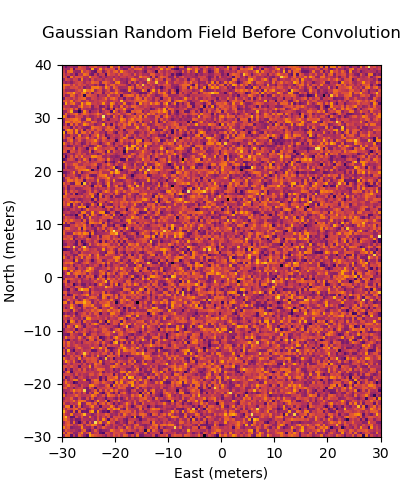
\includegraphics[width=0.5\textwidth]{../images/GRFbeforeConv.png}
				\caption{A Gaussian Random Field (GRF) with values separated by a desired spacing parameter, or resolution}
				\label{CFandEncoder}
			\end{figure}
		\end{minipage}
		\vfill%
		
	\end{frame}

	\begin{frame}[t]{Building a Field}
		\frametitle{Building a Field}
		\framesubtitle{Gaussian Random Field (GRF)}
		\hskip-0.75cm
		\begin{minipage}[t]{0.2\linewidth}\vspace{-0.5cm}
			\tiny\tableofcontents[currentsection,currentsubsection,hideothersubsections,subsectionstyle=show/shaded]
		\end{minipage}
		\hfill%
		\begin{minipage}[t]{0.86\linewidth}\vspace{-0.5cm}
			\begin{flushleft}
				$d_{xy}$ : smallest distance separating any two adjacent random values 
				
				$\underline{\text{x}}$ : $1 \times n$ Vector of x-coordinates, $\left[\begin{array}{cccc}x_0 & x_1 & \dots & x_{n-1}\end{array}\right]$,\\
				$ x_i~=~jd_{xy}, j~\in~\mathbb{Z}$
				
				$\underline{\text{y}}$ : $m \times 1$ Vector of y-coordinates, $\left[\begin{array}{cccc}y_0 & y_1 & \dots & y_{n-1}\end{array}\right]$,\\
				$ y_i~=~jd_{xy}, j~\in~\mathbb{Z}$

				
				$\underline{\text{Z}}$ : $m \times n$ Matrix of z-axis field values 
				
				$\underline{\text{K}}$ : $k \times k$ Matrix representing the kernel for convolution
	
			\end{flushleft}
		\end{minipage}
		\vfill%
		
	\end{frame}
	
	\begin{frame}[t]{Building a Field}
		\frametitle{Building a Field}
		\framesubtitle{Gaussian Random Field (GRF)}
		\hskip-0.75cm
		\begin{minipage}[t]{0.2\linewidth}\vspace{-0.5cm}
			\tiny\tableofcontents[currentsection,currentsubsection,hideothersubsections,subsectionstyle=show/shaded]
		\end{minipage}
		\hfill%
		\begin{minipage}[t]{0.86\linewidth}\vspace{-0.5cm}
			\begin{flushleft}
				A kernel is required to smooth the GRF to better describe some phenomenon. A 2D Gaussian function can be chosen for a Gaussian kernel
				\begin{equation}
					g(x, y) = \frac{1}{2\pi\sigma^2}e^{-\bigg(\frac{(x-\mu_x)^2 + (y-\mu_y)^2}{2\sigma^2}\bigg)}
				\end{equation}
				To form the Gaussian kernel
				\begin{equation}
					
				\end{equation}
			\end{flushleft}
		\end{minipage}
		\vfill%
		
	\end{frame}
	
	\begin{frame}[t]{Building a Field}
		\frametitle{Building a Field}
		\framesubtitle{Gaussian Random Field (GRF)}
		\hskip-0.75cm
		\begin{minipage}[t]{0.2\linewidth}\vspace{-0.5cm}
			\tiny\tableofcontents[currentsection,currentsubsection,hideothersubsections,subsectionstyle=show/shaded]
		\end{minipage}
		\hfill%
		\begin{minipage}[t]{0.86\linewidth}\vspace{-0.5cm}
			\begin{figure}[t]
				\centering
				\captionsetup{width=0.9\textwidth}
				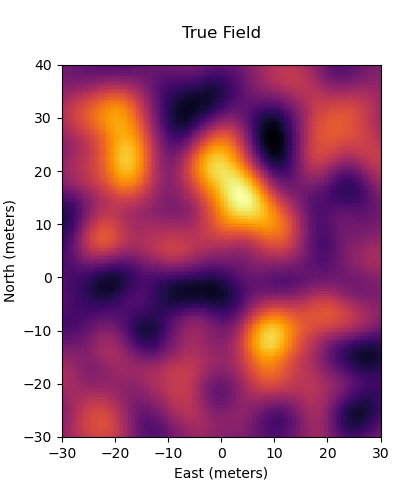
\includegraphics[width=0.5\textwidth]{../images/GRFafterConv.png}
				\caption{A GRF after convolving a 2D Gaussian kernel}
				\label{CFandEncoder}
			\end{figure}
		\end{minipage}
		\vfill%
		
	\end{frame}

	%%%%%%%%%%%%%%%%%%%%%%%%%%%%%%%%%%%%%%%%%%%%%%%%%%%%%%%%%%%%%%%%%%%%%%%%%%%%%%%%%%%%%%%%%%%%%%%
	% Section: Supplemental Material
	%%%%%%%%%%%%%%%%%%%%%%%%%%%%%%%%%%%%%%%%%%%%%%%%%%%%%%%%%%%%%%%%%%%%%%%%%%%%%%%%%%%%%%%%%%%%%%%
	
	\section{Supplemental Material}
	\begin{frame}[t]{Supplemental Material}
		\frametitle{Supplemental Material}
		\framesubtitle{Guidance Navigation and Control: LTP}
		
		\hskip-0.75cm
		\begin{minipage}[t]{0.2\linewidth}\vspace{-0.5cm}
			\tiny\tableofcontents[currentsection,currentsubsection,hideothersubsections,subsectionstyle=show/shaded]
			\vfill%
		\end{minipage}
		\hfill%
		\begin{minipage}[t]{0.86\linewidth}\vspace{-0.5cm}
			Conversion of GPS latitude, longitude, altitude to Earth-Centered Earth-Fixed (ECEF) to NED in a LTP:
			\begin{equation}
			\underline{p}^\text{ECEF} =
			(r_\text{Earth} - a) 
			\begin{bmatrix}
			\cos(\phi) \cos(\lambda)\\
			\cos(\phi) \sin(\lambda)\\
			\sin(\phi)\\
			\end{bmatrix}
			\end{equation}
			
			\begin{equation} 
			\underline{\text{R}} = 
			\begin{bmatrix}
			-\sin(\phi)\cos(\lambda) & -\sin(\lambda) & -\cos(\phi)\cos(\lambda) \\
			-\sin(\phi)\sin(\lambda) & \cos(\lambda) & -\cos(\phi)\sin(\lambda) \\
			\cos(\phi) & 0 & -\sin(\phi)
			\end{bmatrix}
			\end{equation}
			
			\begin{equation}
			\underline{p}^\text{NED} = \underline{\text{R}}^\text{T}(\underline{p}^\text{ECEF} - \underline{p}^\text{Ref})
			\end{equation}
			
			\begin{equation}
			\underline{\text{W}}_i^\text{LTP} = 
			\begin{bmatrix}
			\underline{p}_2^\text{NED} & 
			\underline{p}_1^\text{NED}
			\end{bmatrix}
			=
			\begin{bmatrix}
			E_i & N_i 
			\end{bmatrix}
			\end{equation}
			\vfill%
		\end{minipage}
		
	\end{frame}


	%%%%%%%%%%%%%%%%%%%%%%%%%%%%%%%%%%%%%%%%%%%%%%%%%%%%%%%%%%%%%%%%%%%%%%%%%%%%%%%%%%%%%%%%%%%%%%%
	% Section: References
	%%%%%%%%%%%%%%%%%%%%%%%%%%%%%%%%%%%%%%%%%%%%%%%%%%%%%%%%%%%%%%%%%%%%%%%%%%%%%%%%%%%%%%%%%%%%%%%
%	\section{References}
%	\begin{frame}[allowframebreaks]{Bibliography}
%		\frametitle{References}
%		\bibliographystyle{ieeetr}
%		\bibliography{../../somefolder/some_bib_file}
%		
%	\end{frame}


	%%%%%%%%%%%%%%%%%%%%%%%%%%%%%%%%%%%%%%%%%%%%%%%%%%%%%%%%%%%%%%%%%%%%%%%%%%%%%%%%%%%%%%%%%%%%%%%
	
\end{document}